% Copyright 2026 Sreeram Anil
% SPDX-License-Identifier: CC-BY-4.0
% =============================================================================
%  Gauss-Hermite quadrature Kalman filter — classical Kalman family
% =============================================================================
\chapter{Gauss--Hermite Quadrature Kalman Filter (GHKF)}
\label{ch:ghkf}

\section*{At a glance}
\begin{tabular}{@{}l>{\raggedright\arraybackslash}p{0.76\textwidth}@{}}
Family & classical Kalman (quadrature) \\
Header & \texttt{include/estkit/filters/ghkf.hpp} \\
Registered name & \texttt{GHKF} \\
State dimension & $n_x = 4$ (cell model) --- generic in $n_x, n_u, n_y$ \\
Quadrature points & $m^{n_x} = 3^4 = 81$ (points per axis $m$ is a template parameter) \\
Cost per step & $\mathcal{O}(m^{n_x} n_x^2)$; $11.2$--$12.1\,\SI{}{\micro\second}$/step \\
Primary references & \cite{ito2000gaussian,arasaratnam2007ghqf,wu2006numerical,golubwelsch1969} \\
\end{tabular}

\section{Motivation and aerospace/BMS relevance}
Every filter in this family is an approximation of the same Gaussian-weighted integral
\eqref{eq:ckf-integral}. The unscented, cubature and divided-difference rules all pick a
small, clever point set. The Gauss--Hermite filter of Ito and Xiong~\cite{ito2000gaussian}
instead uses the \emph{optimal} one-dimensional quadrature rule and forms a tensor product:
$m$ points per axis integrate polynomials of degree $\le 2m-1$ exactly, and the accuracy can
be dialled up simply by increasing $m$. It is therefore the natural reference implementation
of a Gaussian filter --- the estimator you run to find out how much of the remaining error is
due to the moment approximation and how much is due to the Gaussian assumption itself.

Its weakness is equally clear: the number of points grows as $m^{n_x}$. For the cell model
($n_x = 4$, $m = 3$) that is $81$ points, which is affordable; for a pack-level or
joint state-parameter model with $n_x = 10$ it would be $59\,049$ and the filter is unusable.
Sparse-grid and pruned variants exist, but the honest role of the GHKF in this report is as a
high-accuracy yardstick against which the $8$-, $9$- and $33$-point rules can be judged.

\section{Problem statement and assumptions}
Model \eqref{eq:ekf-proc}--\eqref{eq:ekf-meas} with additive noise; Gaussian assumed density;
the integrals of interest are \eqref{eq:ckf-integral}. The one additional structural
assumption is that $\mP$ admits a Cholesky factor $\mS$, used to decorrelate the coordinates
so that the $n_x$-dimensional Gaussian factorises into $n_x$ independent standard normals.

\section{Derivation}
\paragraph{One-dimensional rule.} The $m$-point Gauss--Hermite rule for the standard normal
weight is characterised by: nodes $\zeta_1,\dots,\zeta_m$ = roots of the $m$-th probabilists'
Hermite polynomial $He_m$, weights $\omega_j$ chosen so that
\begin{equation}
\int_{\real}\phi(\zeta)\,\frac{e^{-\zeta^2/2}}{\sqrt{2\pi}}\,d\zeta = \sum_{j=1}^m \omega_j\,\phi(\zeta_j)
\qquad\text{exactly for all polynomials } \phi \text{ of degree} \le 2m-1.
\label{eq:ghkf-1d}
\end{equation}
Nodes and weights are the eigenvalues and squared first eigenvector components of the
symmetric tridiagonal Jacobi matrix of the Hermite recurrence (Golub and
Welsch~\cite{golubwelsch1969}); for small $m$ they are available in closed form. For $m=3$,
$He_3(\zeta) = \zeta^3-3\zeta$, so
\begin{equation}
\zeta \in \left\{-\sqrt3,\;0,\;+\sqrt3\right\}, \qquad
\omega \in \left\{\tfrac16,\;\tfrac23,\;\tfrac16\right\}.
\label{eq:ghkf-m3}
\end{equation}
Checking the moments: $\sum\omega_j = 1$, $\sum\omega_j\zeta_j^2 = 2\cdot\tfrac16\cdot3 = 1$,
$\sum\omega_j\zeta_j^4 = 2\cdot\tfrac16\cdot9 = 3$ --- the first three even moments of
$\N{0}{1}$ are exact, and the first failure is at degree six
($\sum\omega_j\zeta_j^6 = 9$ against the true $15$), consistent with exactness to degree
$2m-1=5$. The $m=2$ rule, also tabulated in the header, has nodes $\pm1$ and weights
$\tfrac12$ and is exact to degree three --- it is the one-dimensional ancestor of the
third-degree cubature rule.

\paragraph{Tensor product.} With $\vx = \xhat + \mS\vz$ and $\vz\sim\N{\bm0}{\mI}$, the
$n_x$-dimensional integral factorises and the product rule is
\begin{equation}
\int g(\vx)\N{\vx;\xhat}{\mP}\,d\vx \approx
\sum_{j_1=1}^{m}\cdots\sum_{j_{n_x}=1}^{m}
\left(\prod_{r=1}^{n_x}\omega_{j_r}\right)
g\!\left(\xhat + \mS\,[\zeta_{j_1},\dots,\zeta_{j_{n_x}}]^\T\right),
\label{eq:ghkf-tensor}
\end{equation}
i.e. $N_s = m^{n_x}$ points $\bm{\xi}_s$ with weights $w_s = \prod_r \omega_{j_r}$, all
strictly positive. Because \eqref{eq:ghkf-1d} is exact per axis, \eqref{eq:ghkf-tensor} is
exact for every \emph{multivariate} polynomial whose degree in each individual variable is at
most $2m-1$ --- a stronger statement than the total-degree exactness of the cubature rules,
which is why a $3$-point grid matches a fifth-degree cubature rule and exceeds it on
cross-terms such as $z_1^4z_2^4$.

\paragraph{Filter recursion.} Identical in structure to the CKF, with the equal weights
replaced by $w_s$:
\begin{align}
\mathcal{X}_s &= \xhat + \mS\bm{\xi}_s, &
\xminus_k &= \sum_s w_s f(\mathcal{X}_s,\vu_{k-1}), \label{eq:ghkf-tu1}\\
\Pminus_k &= \sum_s w_s\left(f(\mathcal{X}_s,\vu_{k-1})-\xminus_k\right)(\cdot)^\T + \mQ, &&
\label{eq:ghkf-tu2}
\end{align}
and, after regenerating the grid from $(\xminus_k,\Pminus_k)$,
\begin{align}
\yhat_k &= \sum_s w_s\,h(\mathcal{X}_s,\vu_k), &
\mP_{yy} &= \sum_s w_s(\mathcal{Z}_s-\yhat_k)(\cdot)^\T + \mR, \label{eq:ghkf-mu1}\\
\mP_{xy} &= \sum_s w_s(\mathcal{X}_s-\xminus_k)(\mathcal{Z}_s-\yhat_k)^\T, &
\mK_k &= \mP_{xy}\mP_{yy}\inv, \label{eq:ghkf-mu2}
\end{align}
with $\xplus_k = \xminus_k + \mK_k(\vy_k-\yhat_k)$ and
$\Pplus_k = \Pminus_k - \mK_k\mP_{yy}\mK_k^\T$. Since all $w_s>0$, $\Pminus_k$ and the
subtracted term are both proper covariances and no definiteness safeguard beyond the usual
symmetrisation is needed.

\section{Algorithm}
\begin{algorithm}[H]
\caption{GHKF --- one sampling period (additive noise)}
\begin{algorithmic}[1]
\Require $\xplus_{k-1},\Pplus_{k-1},\vu_{k-1},\vy_k,\vu_k$; grid $\{\bm{\xi}_s,w_s\}_{s=1}^{m^{n_x}}$ precomputed
\State $\mS\gets\operatorname{chol}(\Pplus_{k-1})$;\; $\mathcal{X}_s\gets\xplus_{k-1}+\mS\bm{\xi}_s$
\State \textbf{Time update:} $\mathcal{X}_s\gets f(\mathcal{X}_s,\vu_{k-1})$;\;
       $\xminus_k\gets\sum_s w_s\mathcal{X}_s$;\;
       $\Pminus_k\gets\sum_s w_s(\mathcal{X}_s-\xminus_k)(\cdot)^\T+\mQ$
\State $\mS\gets\operatorname{chol}(\Pminus_k)$;\; $\mathcal{X}_s\gets\xminus_k+\mS\bm{\xi}_s$;\;
       $\mathcal{Z}_s\gets h(\mathcal{X}_s,\vu_k)$;\; $\yhat_k\gets\sum_s w_s\mathcal{Z}_s$
\State $\mP_{yy}\gets\sum_s w_s(\mathcal{Z}_s-\yhat_k)(\cdot)^\T+\mR$;\;
       $\mP_{xy}\gets\sum_s w_s(\mathcal{X}_s-\xminus_k)(\mathcal{Z}_s-\yhat_k)^\T$
\State $\mK\gets\mP_{xy}\mP_{yy}\inv$;\; $\xplus_k\gets\xminus_k+\mK(\vy_k-\yhat_k)$;\;
       $\Pplus_k\gets\Pminus_k-\mK\mP_{yy}\mK^\T$
\State \textbf{if} constraints enabled \textbf{then} $\xplus_k\gets\Pi(\xplus_k)$
\Ensure $\xplus_k,\Pplus_k$
\end{algorithmic}
\end{algorithm}

\section{Application to the battery model}
With $n_x=4$ and $m=3$ the grid has $81$ points. Of these, $16$ have all four coordinates at
$\pm\sqrt3$ (weight $1/1296$ each), $32$ have three (weight $1/324$), $24$ have two
(weight $1/81$), $8$ have one (weight $4/81$) and one is the mean (weight $16/81$). The
SOC axis is therefore sampled at $\soc$ and $\soc\pm\sqrt3\sigma_\soc$, the same stencil as
the DD2 filter of Chapter~\ref{ch:cdkf} --- which is exactly why the two produce identical
results on this problem.

Implementation choice: the number of points per axis is a template parameter,
\code{Ghkf<Model, MPTS>}, with compile-time node/weight tables for $m=2$ and $m=3$ and a
\code{static\_assert} otherwise, plus a second \code{static\_assert} that rejects grids above
$4096$ points. The registered estimator uses \code{Ghkf<EcmModel, 3>}. The grid itself
(abscissae $\bm{\xi}_s$ and weights $w_s$) is built once in the constructor by a mixed-radix
expansion of the grid index and stored as members, so the per-step work is only the affine map
$\xhat + \mS\bm{\xi}_s$ and the model evaluations.

\section{Implementation notes}
$162$ model evaluations per step is the entire cost story: at
$11.2$--$12.1\,\SI{}{\micro\second}$ per step the GHKF is $25\times$ an EKF step and $9\times$ a
CDKF step for identical accuracy.
Zero-coordinate axes are skipped in the affine map (a point with $\xi_r = 0$ contributes
nothing from column $r$ of $\mS$), which saves about a third of the multiply-accumulates in
the point generation. \code{sizeof(Ghkf<EcmModel,3>)} is 10\,784\,bytes --- by far the largest
in this family --- because the $81\times4$ abscissa table, the $81$ weights and the $81$
propagated points are all members; on a memory-constrained MCU this alone rules the filter
out. All weights are positive, so the single-precision build is unproblematic (measured
nominal $\text{RMSE}_{\text{ss}} = 0.02\,\%$ in float against $0.05\,\%$ in double, and
$1.96\,\%$ against $1.84\,\%$ on \texttt{aged\_cell} --- differences at the level of the noise
realisation rather than systematic).

\section{Benchmark results}
\input{tables/cell_GHKF.tex}
\begin{figure}[H]\centering
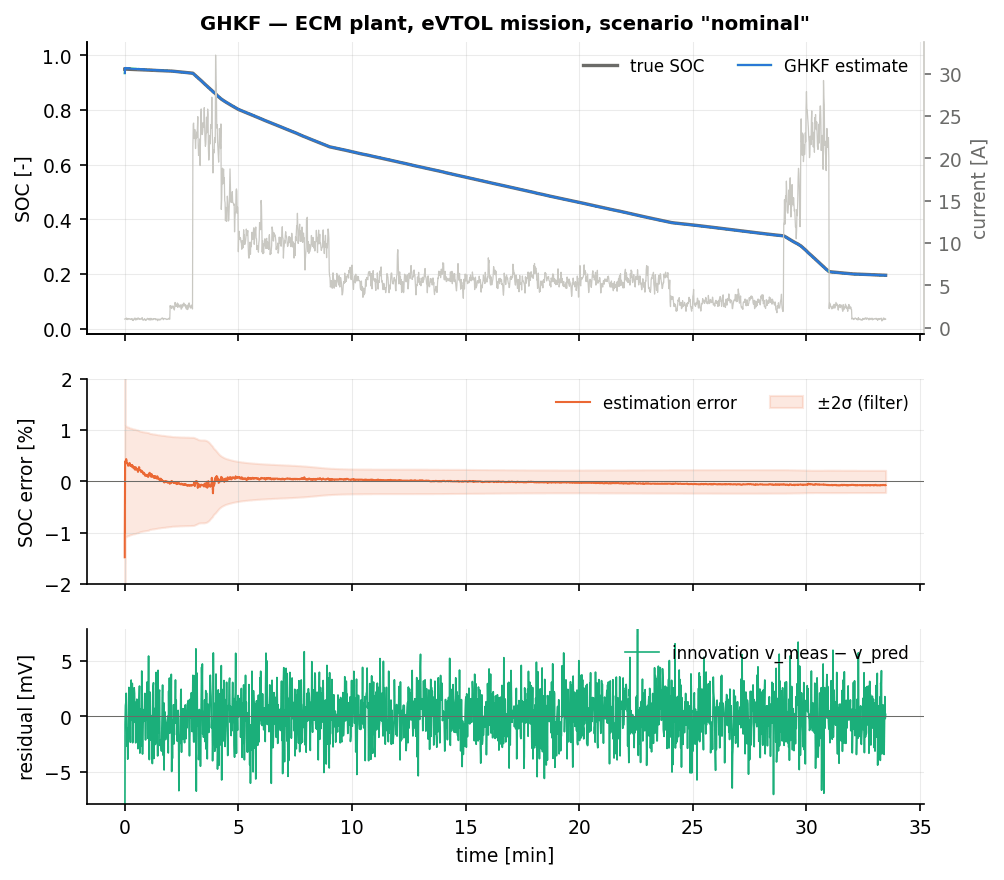
\includegraphics[width=\textwidth]{figures/cell_GHKF_nominal.png}
\caption{GHKF on the nominal eVTOL mission: true and estimated SOC (top), estimation error with the $\pm 2\sigma$ band when available (middle), voltage residual (bottom).}
\end{figure}
\begin{figure}[H]\centering
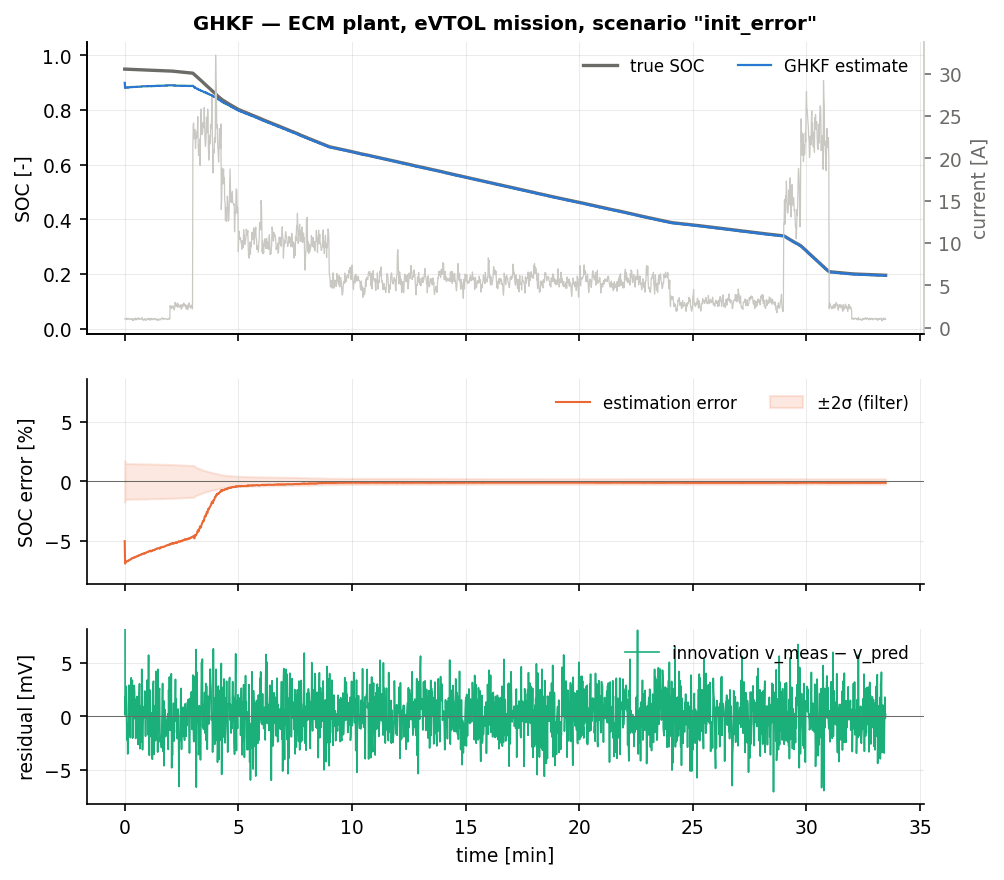
\includegraphics[width=\textwidth]{figures/cell_GHKF_init_error.png}
\caption{GHKF with a 35\,\% initial SOC error.}
\end{figure}

All numbers are three-seed means in per cent SOC.

The GHKF reproduces the CKF5 (Chapter~\ref{ch:ckf5}) and the CDKF (Chapter~\ref{ch:cdkf}) to two
decimal places on all twelve ECM scenarios and all nine SPM scenarios: \texttt{nominal}
$0.08/0.05\,\%$, \texttt{init\_error} $1.85/0.12\,\%$ with $t_{\text{conv}} = 229$\,s,
\texttt{outliers} $0.31/0.08\,\%$, \texttt{aged\_cell} $2.50/1.54\,\%$,
\texttt{param\_mismatch} $1.84/1.79\,\%$, \texttt{sensor\_dropout} $2.75/1.86\,\%$,
\texttt{preisach} $1.27/0.24\,\%$, \texttt{combined} $14.64/11.96\,\%$; SPM \texttt{nominal}
$4.70/4.61\,\%$ and \texttt{cold} $8.74\,\%$. Since the GHKF is the most accurate quadrature of
the three, this agreement is the strongest statement this report can make about the cell
problem: \textbf{beyond fifth-degree exactness there is nothing left to gain from better moment
integration}. Whatever error remains is due to the Gaussian assumption or to model error, not to
the quadrature; a particle filter or a Gaussian-sum filter, not a better cubature rule, would be
the next step.

The corollary is a cost statement. The GHKF pays $11.2$--$12.1\,\SI{}{\micro\second}$ per step
and $10.8$\,kB of state for results that the $9$-point DD2 filter obtains in
$1.28$--$1.39\,\SI{}{\micro\second}$ and $4.3$\,kB --- a factor of nine in time and two and a
half in memory. On this model there is no operating regime in which the GHKF is the right
engineering choice; its value here is diagnostic. That conclusion is specific to $n_x = 4$ and a
mildly nonlinear measurement --- in problems where $g$ has features narrower than $\sigma$,
raising $m$ is the only systematic way to resolve them, and the GHKF is then the only tool in
this chapter that can.

Like every wide-stencil rule it converges slowly from the $-35\,\%$ initial error ($229$\,s)
and from the hysteresis offset of \texttt{preisach} ($217$\,s against the EKF's $16$\,s), it is
well behind the EKF on \texttt{sensor\_dropout} ($1.86\,\%$ against $0.46\,\%$), and it fails
on \texttt{combined} ($11.96\,\%$, never converges) for the reason given in
Chapter~\ref{ch:ckf}: the posterior variance collapses after the first update and the estimate
is subsequently locked in against an unmodelled $25\,\%$ increase in $R_0$. Integrating a wrong
model very accurately does not make it right.

\paragraph{SPM plant: structured model error.}
\begin{figure}[H]\centering
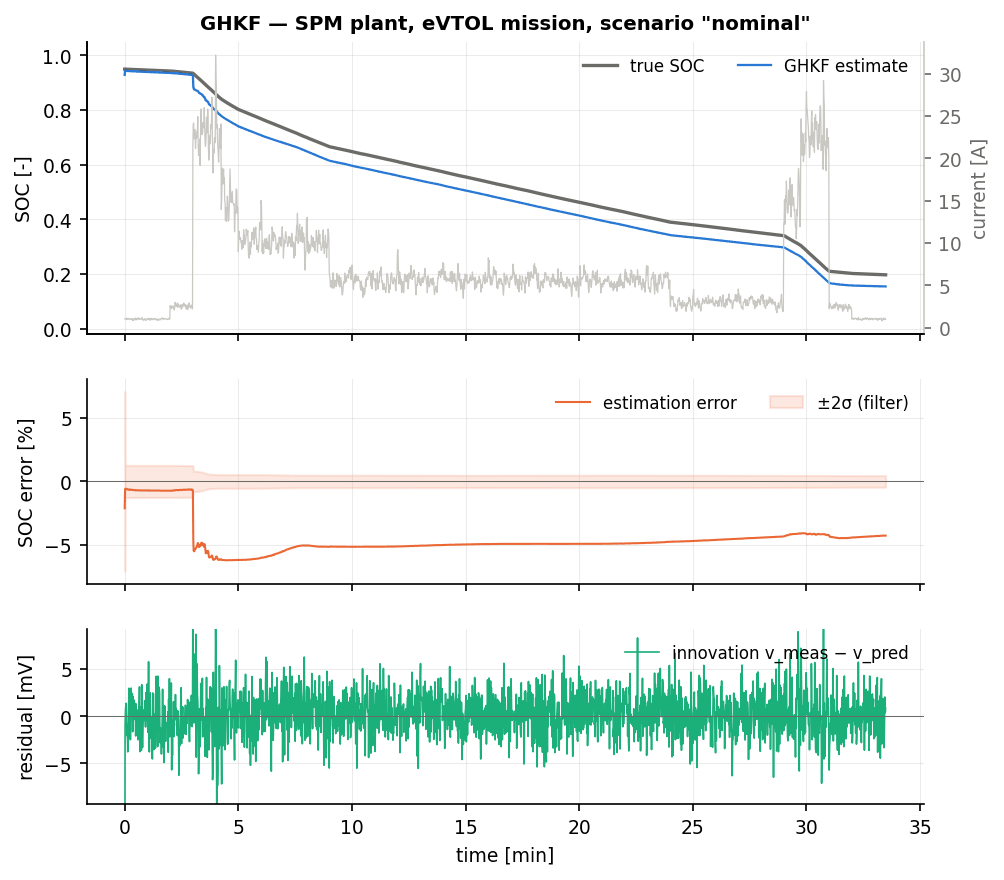
\includegraphics[width=\textwidth]{figures/cellspm_GHKF_nominal.png}
\caption{GHKF on the nominal mission with the electrochemical (SPM) plant.}
\end{figure}
The SPM block of the table is a different kind of test. The plant is the electrochemical
single-particle model; the estimator still runs a 2-RC equivalent circuit, fitted to that plant,
which leaves a \emph{structured} residual of about $4$\,mV (Butler--Volmer kinetics and
solid-phase diffusion that no 2-RC circuit can reproduce) and a slow second branch,
$\tau_2 = 556$\,s. Over a $33$-minute mission a $556$\,s pole barely relaxes, so $v_2(t)$ is
close to an affine ramp --- and so is $\ocv(\soc(t))$ while the cell discharges at a roughly
constant rate. The two channels through which the measurement sees the state,
$(\partial\ocv/\partial\soc)\,\delta\soc$ and $-\delta v_2$, are therefore nearly collinear in
the information accumulated over the flight: the pair $(\soc, v_2)$ is close to unobservable,
and no filter can decide whether a persistent few-millivolt residual belongs to the slow RC
branch or to the state of charge. Because that direction is weakly observable, a $4$\,mV
structured error maps onto \emph{several per cent} of SOC instead of the
$4\,\text{mV}/0.8\,\text{V}\approx0.5\,\%$ a well-conditioned channel would give. This
$(\soc,v_2)$ ambiguity, not the size of the residual, is the mechanism behind the
$3.7$--$4.6\,\%$ band in which the whole classical family sits.

The fifth-degree rules sit at the bad end of the band: $4.61\,\%$ on SPM \texttt{nominal}
against the EKF's $3.73\,\%$ and the LKF's $1.72\,\%$, $8.74\,\%$ on \texttt{cold} against
$7.35\,\%$, $8.24\,\%$ on \texttt{sensor\_dropout} against $5.31\,\%$, $4.90\,\%$ on
\texttt{param\_mismatch} against $3.13\,\%$. They are statistically indistinguishable from the
third-degree CKF ($4.62$, $8.72$, $8.24$, $4.81\,\%$) --- the extra degree of exactness buys
nothing at all here --- and the ordering across the family is monotone in the point spread:
LKF (frozen tangent) $1.72$, EKF/IEKF (tangent at the mean) $3.66$--$3.73$, UKF
($0.2\sigma$ points) $3.96$, the degree-three and degree-five rules ($2\sigma$ and
$2.45\sigma$) $4.61$--$4.62$. The reason is the ambiguity above: a statistical linearisation
over a wide prior returns the \emph{chord} of the OCV curve, which is steeper than the tangent
over most of the mission, so these filters believe the OCV channel is more informative than it
is and commit harder to the direction that carries the structured error. The exception is
\texttt{outliers} ($2.27\,\%$), better than on the ECM plant for everyone because the corrupted
samples widen the effective innovation covariance. Nothing diverges; every SPM error is a bias,
not a drift ($t_{\text{conv}} = 0$ throughout).

The SPM rows make the diagnostic point of this chapter unusually sharply. The GHKF integrates
the Gaussian moments essentially exactly, and it is still $4.6\,\%$ wrong --- worse than the
crudest filter in the family. That is the clearest possible demonstration that the residual
error on the SPM plant is \emph{not} quadrature error: it is the Gaussian assumption meeting a
mis-specified model along a nearly unobservable direction, and no amount of integration
accuracy touches it.

\section{Summary}
The Gauss--Hermite filter is the reference Gaussian filter: tensor-product quadrature, all
weights positive, accuracy set by a single integer $m$, and exactness to degree $2m-1$ in every
variable. Use it to establish how much of a filter's error is quadrature error --- on this
benchmark the answer is ``none beyond degree five'', on either plant --- or on genuinely hard,
strongly nonlinear low-dimensional problems where $m$ must be raised. Do not use it in
production at $n_x\gtrsim6$: $m^{n_x}$ points is a wall, and the DD2 filter of
Chapter~\ref{ch:cdkf} delivers identical results here at one ninth of the cost.
